\section{Network layers and the OSI model}
The task of enabling two or more processes to communicate across physical machines requires a lot of work, and a lot of errors have to be considered, depending on the medium used to transport data. Addressing, both at the process and machine layer has to be handled, and the interface to the physical medium needs to be considered. Grouping problems into logical sections help to solve this problem, as an otherwise very complicated procedure can be broken down into small self contained processes.
One such way of grouping a network framework is the OSI model \cite[27-42]{KOM}. The OSI model is represented as a stack of processes (hereafter referred to as a ''network stack''), which together enables a group of processes to communicate across physical and logical networks.
In itself the OSI model is not an actual network stack, but it is a model of an architecture that is both robust and flexible. 
As seen in Figure \ref{fig:osi_model_stack} it defines seven layers in a networking application, where each layer corresponds to a logical section of the network protocol, and a message passes from the top layer in the first process, potentially all the way to the bottom of the stack, until it has arrived at the second process stack, after which it begins ''climbing'' the stack, and thereby making the message available to the second process.

\begin{figure}[htb]
	\begin{center}
	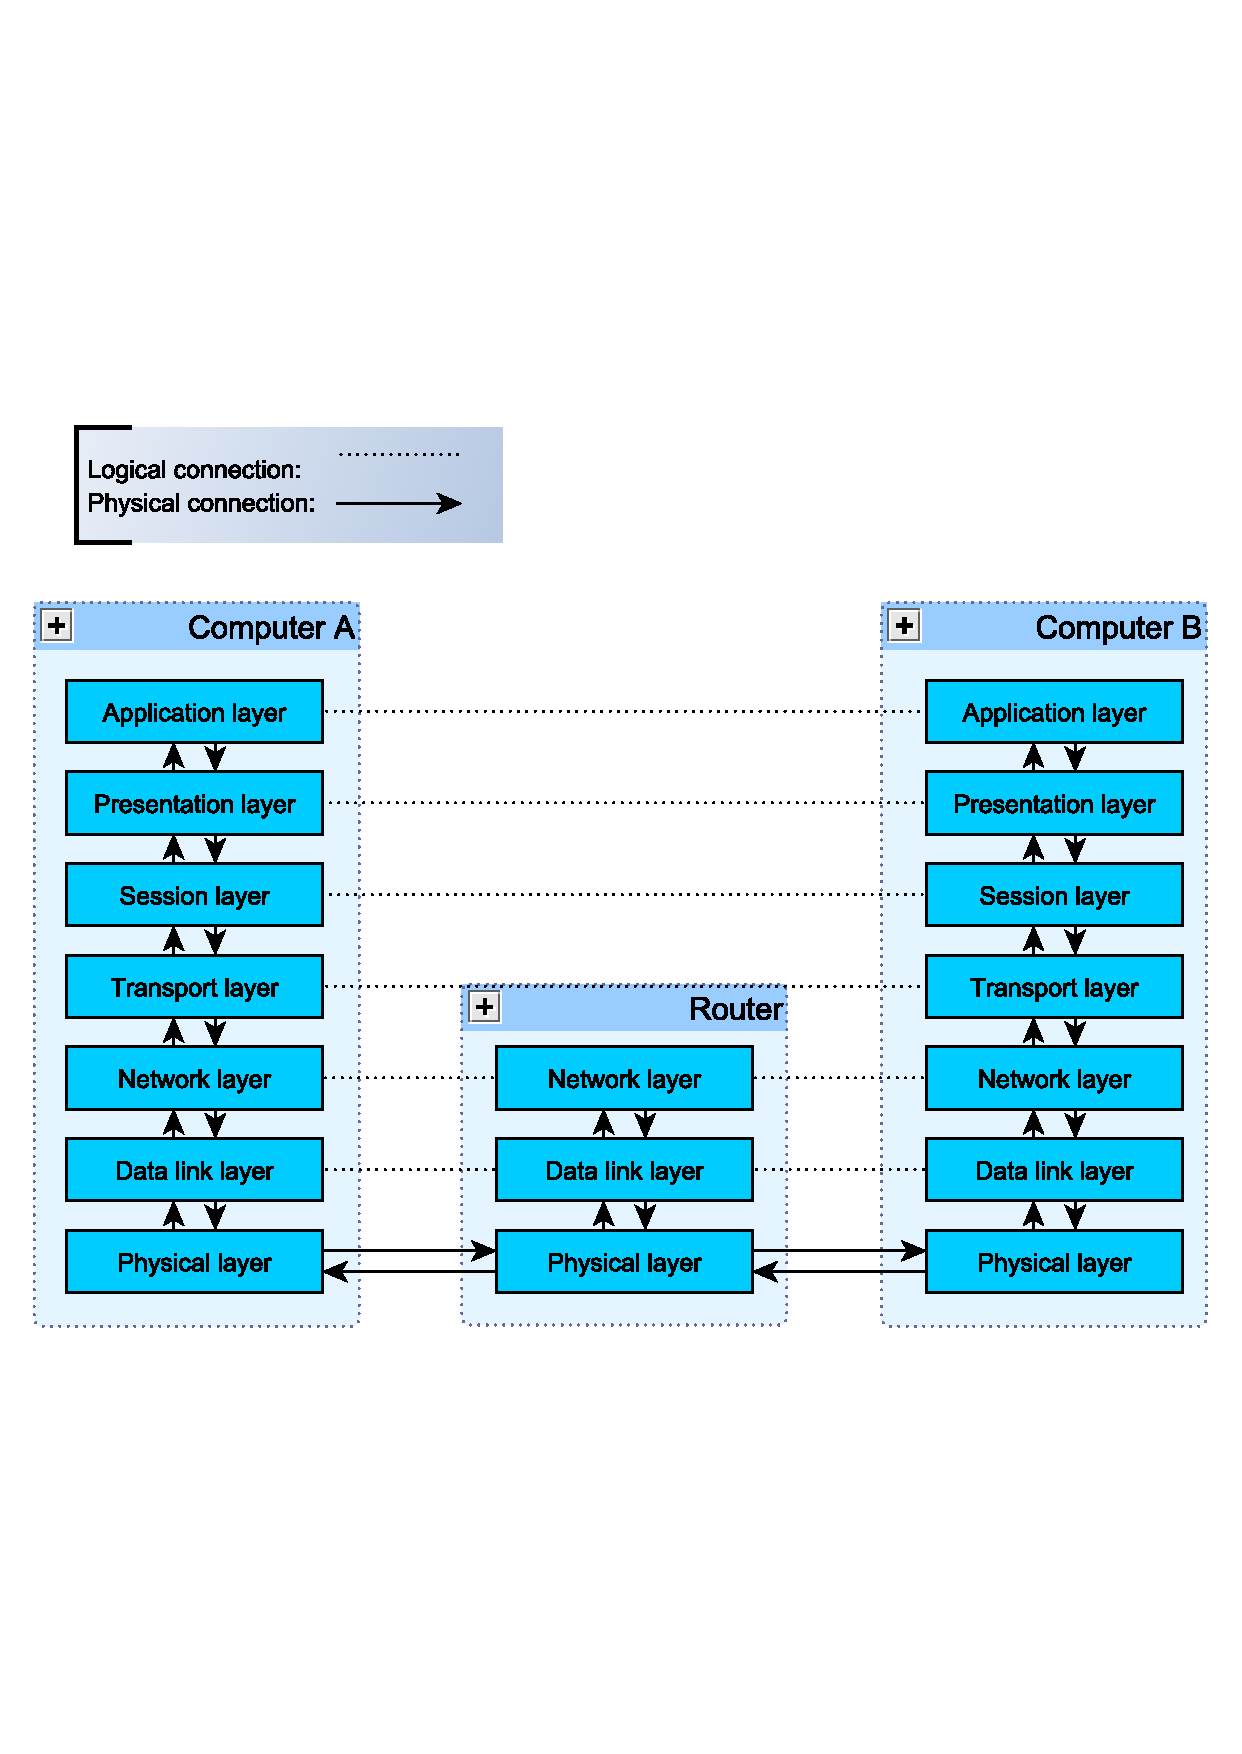
\includegraphics[scale=0.5,trim=0 200 0 200]{content/graphics/OsiStack.pdf} %trim=l b r t (can cut off from every side)
	\caption{OSI model}
	\label{fig:osi_model_stack}			% figure labels are of the form \label{fig:*}
	\end{center}
\end{figure}


Each layer interfaces to the layer above and/or below it, either adding or removing data from the package that is passed. This is either done directly, or by a third-party control mechanism depending on the choice of architecture.
Layer one, two and three can be considered the network support layer, they are responsible for ensuring dataflow through the network of physical machines and they are expected to be active and usable, even though no client application is using the network on a machine.

\subsection{Physical layer}
This layers responsibility is to enable a stream of bits to be broadcast between physical machines, typically through a wire, by the means of electricity or in this case through air, by means of sound. Synchronization, encoding and the transmission speed, are all things that the physical layer needs to handle.

\subsection{Data link layer}
The data link layer uses the physical layer to present an error free transmission line. Data coming from the higher layers, is divided into frames (small manageable units) which the physical layer can handle. Local addressing is also handled by the data link layer.

\subsection{Network layer}
The network layer is responsible for package routing across larger networks, especially across networks where the sender isn't directly connected to the receiver. It handles sending and receiving arbitrarily large blocks of data from and to the higher layers.

\subsection{Transport layer}
The transport layer ensures that a process can deliver a package to another process, thus making sure packages arrives in order and intact.

\subsection{Session layer}
This layer handles synchronization between two network processes, and dialog control (whether communication should be full duplex or half duplex).

\subsection{Presentation layer}
The presentation layer is concerned with ensuring that the data is interpreted correctly (int, float, string. etc), encryption and compression.

\subsection{Application layer}
This is the final application, using the network stack. For instance a chat client, email client etc.
